\documentclass[10pt,presentation]{beamer}

%%
%% RWTH Beamer Theme (layout based on RWTH PowerPoint template)
%% by Georg Wassen, Lehrstuhl für Betriebssysteme, 2013
%%    wassen@lfbs.rwth-aachen.de
%% with modifications by Gerrit Toehgiono, Mentoring Informatik, 2016-2018
%% to match the "current old" RWTH template
%%
%% modified for internal use by Mark E. Fuller, RWTH - PCFC, 2020
%%
%% The templates are derived from the beamer documentation and the provided templates,
%% hence, the same licence applies:
%%
%% ----------------------------------------------------------------
%% |  This file may be distributed and/or modified                |
%% |                                                              |
%% |  1. under the LaTeX Project Public License and/or            |
%% |  2. under the GNU Public License.                            |
%% |                                                              |
%% |  See the file doc/licenses/LICENSE for more details.         |
%% ----------------------------------------------------------------
%%
%% Version 0.1    20.12.2012    Initial presentation using this theme
%% Version 0.2    08.01.2013    Extracted layout and some example slides
%% Version 0.3    12.01.2013    Improved handling of \subsection (used as frame title),
%%                              Support institute's logo
%% Version 0.4    22.01.2013    Improved spacing between lines in header & footer
%% Version 0.5    01.02.2013    No right sidebar: set width correctly
%% Version 1.0    06.03.2014    Initial Tag on GitHub
%%
%% Version 1.1    31.03.2018    Modifications for CS Mentoring
%%
%%  - copyright of slides?
%%  - count slides with same subsection (needs probably overloading \subsection) and print: 1/N
%%    (needs to count the number of frames in each subsection)
%%
%% Version 1.1a   31.03.2020    Fork by M.E. FULLER (RWTH - PCFC)

%%%%%%%%%%%%%%%%%%%%%%%%%%%%%%%%%%%%%
%% Select input file encoding:
%%   utf8   - UTF-8, nowadays standard on most operating sytems
%%   latin1 - ISO-8859-1
\usepackage[utf8]{inputenc}

%%%%%%%%%%%%%%%%%%%%%%%%%%%%%%%%%%%%%
%% Select language
%%
%\usepackage[ngerman]{babel}        % Deutsch, neue Rechtschreibung
\usepackage[english]{babel}       % English

\usetheme{rwth}
\usepackage[T1]{fontenc}           % Font encoding (don't change!)
\usepackage{lmodern}               % Select Linux Modern Fonts (don't change)
\usepackage{sansmathfonts}         % Sans fonts in math environments
\usepackage{textcomp}              % fix 'missing font symbols' warning
\renewcommand{\rmdefault}{phv}     % Arial like (Helvetica)
\renewcommand{\sfdefault}{phv}     % Arial like (Helvetica)

%% graphics related packages
\usepackage{graphicx}              % needed to include graphics (don't change)
\usepackage{epstopdf}              % required to include eps files
%\usepackage{svg}                   % include svg files (requires Inkscape)
\usepackage[encoding,filenameencoding=utf8]{grffile} % allow utf8 file names in graphics

%%%%%%%%%%%%%%%%%%%%%%%%%%%%%%%%%%%%%
%% import packages for content
%%
\usepackage{listings}                           % for lstlisting and \lstinline|..|
%% TikZ can be used to /program/ graphics.
\usepackage{tikz}                                % comment-out, if you don't need this.
%% some TikZ-libraries and settings for the examples...
\usetikzlibrary{shadings}           % GW: color gradients
\usetikzlibrary{arrows,calc,positioning,fit,matrix,shadows,chains,arrows,shapes,spy,fadings}
\usepackage{pgfplots}
\usetikzlibrary{pgfplots.units,shapes.symbols,shapes.arrows}
%\usetikzlibrary{pgfplots.external}
%\tikzexternalize[prefix=tmp/]

%% Custom packages and definitions

% Mathematikumgebung
\usepackage{amsmath}
\usepackage{amssymb}
\usepackage{sansmath}

% tabularx -> bessere "tabular"-Umgebung
\usepackage{tabularx}

% zusätzliche Formatbezeichner für die tabularx-Umgebung
\newcolumntype{L}{>{\raggedright\let\newline\\\arraybackslash\hspace{0pt}}X}
\newcolumntype{R}{>{\raggedleft\let\newline\\\arraybackslash\hspace{0pt}}X}
\newcolumntype{C}{>{\centering\let\newline\\\arraybackslash\hspace{0pt}}X}

% center text vertically in tabularx(column)
%\renewcommand{\tabularxcolumn}[1]{>{\large}m{#1}}

% Bessere Tabellenlinien
\usepackage{booktabs}

% Tabellenzeilen für booktabs anpassen -> call on frame with table
\newcommand{\fixbooktabsrowhight}{%
  \setlength{\aboverulesep}{0pt}
  \setlength{\belowrulesep}{0pt}
  \setlength{\extrarowheight}{.5ex}
}

% Zellen über mehrere Zeilen
\usepackage{multirow}

% Source, e.g. for images
\setbeamercolor{framesource}{fg=gray}
\setbeamerfont{framesource}{size=\tiny}

\usepackage[absolute,overlay]{textpos}
\newcommand{\source}[1]{\begin{textblock*}{\linewidth}(1ex,\paperheight-2.75em)
  \begin{beamercolorbox}[left]{framesource}
    \usebeamerfont{framesource}\usebeamercolor[fg]{framesource} Source: {#1}
  \end{beamercolorbox}
\end{textblock*}}

\usepackage{etoolbox}
%% short titles for toc \(sub)section[SHORTTITLE for toc]{LONGTITLE for slide}
\makeatletter
% Insert [short title] for \section in ToC
\patchcmd{\beamer@section}{{#2}{\the\c@page}}{{#1}{\the\c@page}}{}{}
% Insert [short title] for \section in Navigation
\patchcmd{\beamer@section}{{\the\c@section}{\secname}}{{\the\c@section}{#1}}{}{}
% Insert [short title] for \subsection in ToC
\patchcmd{\beamer@subsection}{{#2}{\the\c@page}}{{#1}{\the\c@page}}{}{}
% Insert [short title] for \subsection  in Navigation
\patchcmd{\beamer@subsection}{{\the\c@subsection}{#2}}{{\the\c@subsection}{#1}}{}{}
\makeatother

%% MEF packages and commands
\usepackage{multicol}
\usepackage[version=3]{mhchem} % Formula subscripts using \ce{}
\newcommand{\nox}{NO$_x$} % our abbreviation

%get proper bib with numbered entries
\setbeamertemplate{bibliography item}{\insertbiblabel}

%footnote citations - replace \cite with \footcite or \footfullcite
\usepackage[backend=bibtex, style=authoryear-comp]{biblatex} %, style=authoryear-comp
\addbibresource{references}
\addbibresource{ownpubspres}

%shrink citations
\setbeamerfont{footnote}{size=\tiny}

%no ``figure'' in caption
\setbeamertemplate{caption}{\insertcaption} 

\newcommand{\red}[1]{\textcolor{red}{#1}} %easy red text


\title[Introduction to \textsc{MESS}]{PCFC QM Subgroup:\\An introduction to \textsc{MESS}}
%\subtitle{Subtitle}
%\titlegraphic{}
\author{Mark E. Fuller}
\email{fuller@pcfc.rwth-aachen.de} % optionally
\institute{Physico-Chemical Fundamentals of Combustion}
%\webaddress{www.informatik.rwth-aachen.de/mentoring} % overrides www.rwth-aachen.de
\date{\today}
\subject{RWTH presentation template}
\keywords{RWTH, Latex Beamer, template}

%\logo{\includegraphics[height=8mm]{logos/logo}} % will replace the default logo

% official institute logo offset correction
%\logo{\vskip-3.5mm\includegraphics[height=12.5mm]{logos/rwth_mentoring_rgb.eps}\hspace{-2mm}} % optionally
\logo{\vskip-2mm
\includegraphics[width=45mm]{logos/PCFC.png}\hspace{-2mm}} % optionally

% alternative logo position (not recommended)
%\instlogo{\includegraphics[height=10mm]{logos/rwth_mentoring_rgb.eps}} % optionally

%%%%%%%%%%%%%%%%%%%%%%%%%%%%%%%%%%%%%
%% configure template behaviour
%%-------------------------------
%%   secstart -- style of section start
%%               selectable parameters:
%%                 sectitle:  only provides section title
%%                 sectoc:    display section table of contents
%%                 <empty>:   display nothing on section start
\secstart{sectitle}
% disable PDF navigation icons
\setbeamertemplate{navigation symbols}{}

\begin{document}

\begin{frame}{What is \textsc{MESS}?}
  \begin{itemize}
   \item \textsc{MESS} is the \textbf{M}aster \textbf{E}quation \textbf{S}ystem \textbf{S}olver\footfullcite{Georgievskii.2013}, a component of the \textsc{PAPR} suite of chemical kinetics codes
    \begin{itemize}
     \item Developers: Y. Georgievskii, C. F. Goldsmith, J. A. Miller, M. P. Burke, and S. J. Klippenstein 
     \item \url{https://tcg.cse.anl.gov/papr/codes/mess.html}
    \end{itemize}
   \item Conformers on a potential energy surface are connected via transition states
   \item Ab initio calculations provide necessary input information to calculate partition functions and determine rates via transition state theory (TST)
  \end{itemize}
\end{frame}

\begin{frame}{\ce{H2N1O2} Potential Energy Surface\footfullcite{Fuller.2018}}
%\begin{multicols}{2}
  \begin{itemize}
   \item System consists of three kinds of nodes (conformers):
    \begin{itemize}
     \item \textsc{Bimolecular}: a pair of fragments which are lumped together, \textit{e.g.} \ce{H}+\ce{HNO2}
     \item \textsc{Well}: a unimolecular intermediate, \textit{e.g.} \ce{HONOH}
     \item \textsc{Barrier}: a transition state (TS) between two wells/bimoleculars
    \end{itemize}
   \item Each conformer is described by its geometry and frequencies and (relative) energy
  \end{itemize}
%  \columnbreak
  \begin{figure}
    \centering
    %tex file to generate this figure in figures folder
    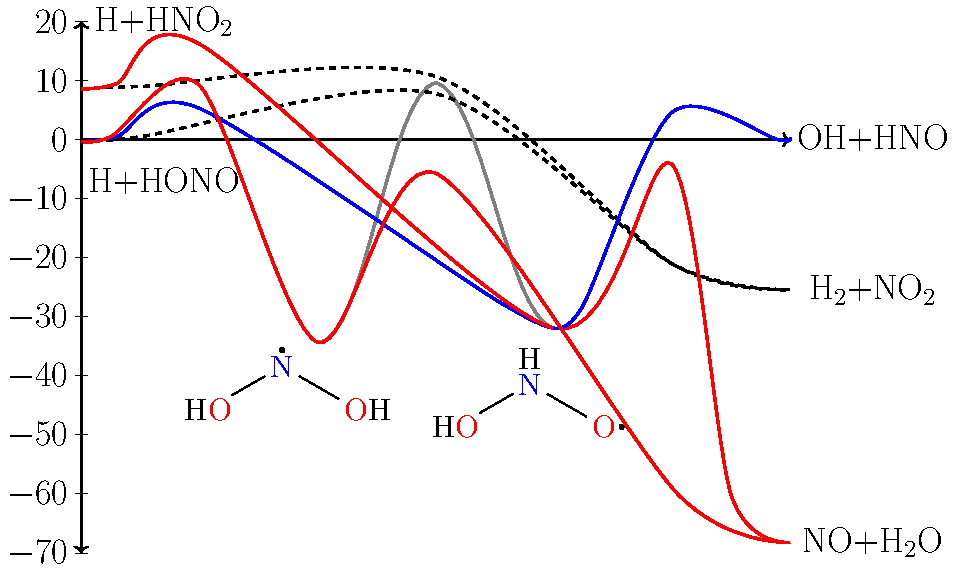
\includegraphics[width=0.6\linewidth]{figures/PES_H_HONO_1_lumpHONO.pdf}
  \end{figure}
%\end{multicols}
\end{frame}

\section{MESS Input File}
% /home/fuller/Documents/PCFC/Pubs_Pres/QMsubgroup/20200512_MESS/MESS_Version0/Current/h2no2_b2plypd3_ccpvtz_lhono_0.inp
% \lstinputlisting[language=Python, linerange={37-45,48-50}]{source_filename.py}
% \lstinputlisting[language=Python, firstline=37, lastline=45]{source_filename.py}
%
% This requires the package listings
% 
% Slides containing lstlisting environments, \lstinline|..| or \verb|..|
% the option "fragile" must be provided!  /home/fuller/Documents/PCFC/Pubs_Pres/QMsubgroup/20200512_MESS/
% 


\begin{frame}{Input file overview}
  \begin{itemize}
   \item Global section (unnamed header) specifies parameters for solution of the master equation
   \item Specify temperatures, pressures, calculation parameters
   \item Two major choices for calculation method
    \begin{itemize}
     \item \textsc{direct}: fuller, more expensive calculations (not so good at low temperature)
     \item \textsc{low-eigenvalue}: assume which eigenvalues are chemical and which are relaxational, numerically cheap, not accurate at high temperatures
    \end{itemize}
   \item \textsc{Model} definition follows and begins with collision parameters
   \item All conformers are then described to define system
  \end{itemize}
\end{frame}

\begin{frame}[fragile]{Header Information}
  \tiny{
  \lstinputlisting[lastline=22]{MESS/h2no2_b2plypd3_ccpvtz_lhono_0.inp}
  }
\end{frame}

\begin{frame}[fragile]{Bimolecular Input}
  \vspace{-0.8cm}
  \tiny{
  \lstinputlisting[firstline=24,lastline=60]{MESS/h2no2_b2plypd3_ccpvtz_lhono_0.inp}
  }
\end{frame}

\begin{frame}[fragile]{Well Input}
  \vspace{-0.8cm}
  \tiny{
  \lstinputlisting[firstline=248,lastline=284]{MESS/h2no2_b2plypd3_ccpvtz_lhono_0.inp}
  }
\end{frame}

\begin{frame}[fragile]{Barrier Input}
  \vspace{-0.8cm}
  \tiny{
  \lstinputlisting[firstline=288,lastline=323]{MESS/h2no2_b2plypd3_ccpvtz_lhono_0.inp}
  }
\end{frame}

\begin{frame}{Generating \textsc{MESS} Input Blocks}
  \begin{itemize}
   \item While you could, it is tedious and error-prone to write input files manually
   \item The utility program \textsc{writemess} reads a \textsc{Gaussian} output (log) file and writes a conformer template
   \item Optionally, hindered rotors (\textsc{Gaussian} log files) and energy from a single-point calculation (\textsc{ORCA}, currently) may also be added and written concurrently
  \end{itemize}
\end{frame}

\section{Getting Results}
\begin{frame}{Job Submission and Output}
  \begin{itemize}
   \item Assuming everything is installed correctly, job submission on the HPC with slurm is simple: we call \textsc{mess} on the input file
   \begin{itemize}
    \item If we have an input file for a network of bimoleculars, wells, and barriers, then we call \textsc{mess} on the input file
    \item For two bimoleculars connected by a single transition state, we call \textsc{abstraction} on the input file
   \end{itemize}
   \item A log file and output file will be generated by \textsc{MESS}
   \item Output file can be split into three sections:
    \begin{enumerate}
     \item System network at the top
     \item Rate tables at each temperature and pressure condition
     \item Rate tables for each species pair
    \end{enumerate}
   \item The output file requires conversion to a recognized format for inclusion in chemical kinetic mechanisms
  \end{itemize}
\end{frame}

\begin{frame}{Fitting the Output}
  \begin{itemize}
   \item A function to fit the output data to pressure-dependent, modified Arrhenius expressions is posted on the \textsc{MESS} webpage, \url{http://tcg.cse.anl.gov/papr/codes/mess/mess_aux/mod_arr.tgz}
   \item You will likely need to make some small changes for your specific system, but this will output \textsc{CHEMKIN}-format \textsc{PLOG} fits for all of the conformer pairs
  \end{itemize}
\end{frame}

\begin{frame}{Additional Resources}
  \begin{itemize}
   \item The \textsc{MESS} manual: \url{http://tcg.cse.anl.gov/papr/codes/mess/messmanual_3_23_16.pdf}
   \item More examples to run and test: \url{http://tcg.cse.anl.gov/papr/codes/mess/MESS_Examples.tgz}
  \end{itemize}
\end{frame}



% 
% Table of contents (automatically collects all \section{} and \subsection{} entries).
% (run pdflatex multiple times to get all cross references correct)
% 
% \begin{frame}[t]{Agenda}
% \begin{multicols}{2}
%   \tableofcontents[hideallsubsections]
% \end{multicols}
% \end{frame}
% 
% \section{Example slides}
% 
% \begin{frame}{Titel der Folie, der auch in die zweite Zeile laufen darf.}
%   \begin{itemize}
%     \item Liste mit Aufzählungszeichen
%     \item Liste mit Aufzählungszeichen
%       \begin{itemize}
%         \item Zweite Ebene
%           \begin{itemize}
%             \item Optionale dritte Ebene
%           \end{itemize}
%       \end{itemize}
%     \item Liste mit Aufzählungszeichen
%     \item Liste mit Aufzählungszeichen
%       \begin{itemize}
%         \item Zweite Ebene
%       \end{itemize}
%   \end{itemize}
% \end{frame}
% 
% \begin{frame}{Noch eine Folie mit Aufzählungen}
%   \begin{enumerate}
%     \item Erster Punkt
%       \begin{enumerate}
%         \item Erster Unterpunkt
%         \item Zweiter Unterpunkt
%       \end{enumerate}
%     \item Zweiter Punkt
%       \begin{itemize}
%         \item Erster regulärer Unterpunkt
%         \item Zweiter regulärer Unterpunkt
%       \end{itemize}
%   \end{enumerate}
% \end{frame}
% 
% \begin{frame}{Titel der Folie mit Absätzen}
%   \begin{itemize}
%     \item Lorem ipsum dolor sit amet, consectetur adipisicing elit, sed do eiusmod tempor incididunt ut labore et dolore magna aliqua.
%     \item Lorem ipsum dolor sit amet, consectetur adipisicing elit, sed do eiusmod tempor incididunt ut labore et dolore magna aliqua.
%     \item Lorem ipsum dolor sit amet, consectetur adipisicing elit, sed do eiusmod tempor incididunt ut labore et dolore magna aliqua.
%   \end{itemize}
% \end{frame}
% 
% \begin{frame}{Folie mit Boxen}
%   \begin{block}{Block 1}
%     Inhalt der ersten Box
%   \end{block}
%   \begin{block}{weitere Box}
%     Lorem ipsum dolor sit amet, consectetur adipisicing elit, sed do eiusmod tempor incididunt ut labore et dolore magna aliqua.
%   \end{block}
% \end{frame}
% 
% 
% 
% \section{more Examples}
% 
% 
% If a \subsection{} is available, that one is used as first line of the frame title.
% 
% \subsection{a Subsection}
% 
% \begin{frame}{How to set columns}
%   
%   The columns environment is provided by beamer,
%   see "texdoc beamer", Sec. 12.7 'Splitting a Frame into Multiple Columns'
%   
%   parameter: c - center columns vertically
%              t - align columns on the baseline of the first line
%                  don't use, if a column contains (only) a graphic!
%              T - align columns on the top of the first line (ok with graphics)
%              b - align columns on the bottom line
%   \begin{columns}[T]
%     Each column must be given a with.
%     Should be given relative to \textwidth:
%     \begin{column}{.45\textwidth}
%       \begin{itemize}
%         \item Item 1
%         \item Item 2
%         \item Item 3
%         \item Lorem ipsum dolor sit amet, consectetur adipisicing elit, sed do eiusmod tempor incididunt ut labore et dolore magna aliqua.
%       \end{itemize}
%     \end{column}
%     \begin{column}{.45\textwidth}
%       here, \textwidth is the with of the current column
%       \includegraphics[width=.9\textwidth]{figures/Tux}
%     \end{column}
%   \end{columns}
% \end{frame}
% 
% 
% \begin{frame}{How to set columns (2)}
%   Lorem ipsum dolor sit amet, consectetur adipisicing elit, sed do eiusmod tempor incididunt ut labore et dolore magna aliqua.
%   \begin{columns}[t]
%     \begin{column}{.4\textwidth}
%       \begin{itemize}
%         \item cat
%         \item dog
%         \item mouse
%         \item elephant
%       \end{itemize}
%     \end{column}
%     \begin{column}{.6\textwidth}
%       \begin{itemize}
%         \item Lorem ipsum dolor sit amet, consectetur adipisicing elit, sed do eiusmod tempor incididunt ut labore et dolore magna aliqua.
%         \item Lorem ipsum dolor sit amet, consectetur adipisicing elit, sed do eiusmod tempor incididunt ut labore et dolore magna aliqua.
%       \end{itemize}
%     \end{column}
%   \end{columns}
% 
%   Lorem ipsum dolor sit amet, consectetur adipisicing elit, sed do eiusmod tempor incididunt ut labore et dolore magna aliqua.
% \end{frame}
% 
% \subsection{another subsection}
% 
% \begin{frame}
%   This frame does not contain a (dedicated) frame title.
% \end{frame}
% 
% \section{Examples with uncovering}
% 
% \begin{frame}{Piecewise uncovering using pause}
%   Paragraphs and items can be uncovered easily with \texttt{\textbackslash pause}.
%   \pause
%   \begin{itemize}
%     \item Lorem ipsum dolor sit amet, consectetur adipisicing elit, sed do eiusmod tempor incididunt ut labore et dolore magna aliqua.
%       \pause
%     \item Lorem ipsum dolor sit amet, consectetur adipisicing elit, sed do eiusmod tempor incididunt ut labore et dolore magna aliqua.
%       \pause
%     \item Lorem ipsum dolor sit amet, consectetur adipisicing elit, sed do eiusmod tempor incididunt ut labore et dolore magna aliqua.
%       \pause
%     \item Lorem ipsum dolor sit amet, consectetur adipisicing elit, sed do eiusmod tempor incididunt ut labore et dolore magna aliqua.
%   \end{itemize}
% \end{frame}
% 
% \begin{frame}{Fine grained control}
%   \begin{itemize}
%     \item<1-> First line
%     \item<2>  Second line (appears after first line, disappears again)
%     \item<3-4> Third line (appears before firth one)
%     \item<4-> Fouth line
%     \item<5-> Fifth line
%   \end{itemize}
%   \onslide<6->{
%     Standard behavior with \texttt{\textbackslash onslide} is to keep its place, even if not displayed.
%   }
% 
%   \only<7>{
%     With \texttt{\textbackslash only}, the element does not occupy place. This may lead to shifting other elements.
%   }
% \end{frame}
% 

% 
% 
% 
% 
% \section{TikZ example}
% 
% 
% This requires the package tikz
% 
% The animation uses the same overlay specification<2-3> as the items or \onslide
% 
% \begin{frame}{animated graphics}
% 
%   define some styles
%   \tikzstyle{format} = [draw, thin, fill=blue!20]
%   \tikzstyle{medium} = [ellipse, draw, thin, fill=green!20, minimum height=2.5em]
% 
%   \begin{figure}
%     \begin{tikzpicture}[node distance=3cm, auto,>=latex', thick]
%       We need to set a bounding box first. Otherwise the diagram
%       will change position for each frame.
%       \path[use as bounding box] (-1,0) rectangle (10,-2);
%       \path[->]<1-> node[format] (tex) {.tex file};
%       \path[->]<2-> node[format, right of=tex] (dvi) {.dvi file}
%         (tex) edge node {\TeX} (dvi);
%       \path[->]<3-> node[format, right of=dvi] (ps) {.ps file}
%         node[medium, below of=dvi] (screen) {screen}
%         (dvi) edge node {dvips} (ps)
%         edge node[swap] {xdvi} (screen);
%       \path[->]<4-> node[format, right of=ps] (pdf) {.pdf file}
%         node[medium, below of=ps] (print) {printer}
%         (ps) edge node {ps2pdf} (pdf)
%         edge node[swap] {gs} (screen)
%         edge (print);
%       \path[->]<5-> (pdf) edge (screen)
%         edge (print);
%       \path[->, draw]<6-> (tex) -- +(0,1) -| node[near start] {pdf\TeX} (pdf);
%     \end{tikzpicture}
%   \end{figure}
% 
% \end{frame}


%%%%%%%%%%%%%%%%%%%%%%%%%%%%%%%%%%%%%%%%%%%%%%%%%%%%%%%%%%%%%%%%%%%%%%%%%%%%%%%%%%%%%%%%%%%%%%%%%%%%%%%%%%%%%%%%%%%%%%%%%%%%%%%%%%%%%%%%%%%%
%%%%%%%%%%%%%%%%%%%%%%%%%%%%%%%%%%%%%%%%%%%%%%%%%%%%%%%%%%%%%%%%%%%%%%%%%%%%%%%%%%%%%%%%%%%%%%%%%%%%%%%%%%%%%%%%%%%%%%%%%%%%%%%%%%%%%%%%%%%%

% 
% \begin{frame}{Titel der Folie, der auch in die zweite Zeile laufen darf.}
%  \begin{itemize}
%    \item Liste mit Aufzählungszeichen
%    \item Liste mit Aufzählungszeichen
%      \begin{itemize}
%        \item Zweite Ebene
%          \begin{itemize}
%            \item Optionale dritte Ebene
%          \end{itemize}
%      \end{itemize}
%    \item Liste mit Aufzählungszeichen
%    \item Liste mit Aufzählungszeichen
%      \begin{itemize}
%        \item Zweite Ebene
%      \end{itemize}
%  \end{itemize}
% \end{frame}
% 
% \begin{frame}{Titel der Folie mit Absätzen}
%  \begin{itemize}
%    \item Lorem ipsum dolor sit amet, consectetur adipisicing elit, sed do eiusmod tempor incididunt ut labore et dolore magna aliqua.
%    \item Lorem ipsum dolor sit amet, consectetur adipisicing elit, sed do eiusmod tempor incididunt ut labore et dolore magna aliqua.
%    \item Lorem ipsum dolor sit amet, consectetur adipisicing elit, sed do eiusmod tempor incididunt ut labore et dolore magna aliqua.
%  \end{itemize}
% \end{frame}
% 
% \section[TOC-Titel]{Section-Titel}
% 
% \begin{frame}{Test}
%  Test
% \end{frame}
% 
% \begin{frame}
%  \begin{itemize}
%    \item Punkt 1
%    \item Punkt 2
%    \item Punkt 3
%  \end{itemize}
% \end{frame}
% 
% \begin{frame}
%  \begin{tikzpicture}
%    \node[draw] {Hello, world};
%  \end{tikzpicture}
% \end{frame}
% 
% \begin{frame}{Optionaler Titel der Folie mit Bild}
% \centerline{%
%  \includegraphics[width=\textwidth]{logos/rwth}
%  }
% \end{frame}

\end{document}
